\documentclass[paper=a4, fontsize=12pt, line_length=16cm, number_of_lines=33,dvipdfmx]{jlreq}
%\documentclass[pandoc,12pt]{bxjsarticle}

\usepackage{amsmath,amssymb}
\usepackage[deluxe,uplatex]{otf}
%% Fonts
\usepackage[T1]{fontenc}
\usepackage{tgtermes,tgheros,tgcursor}
\renewcommand{\bfdefault}{bx}
\usepackage[libertine]{newtxmath}
\usepackage{hyperref}
\usepackage{pxjahyper}

\usepackage{graphicx}
\graphicspath{{fig/}}

\usepackage{physics}



\numberwithin{equation}{section}

%%%%%%%%%%%%%%%%%%%%%%%%%%%%%%%%%%%%%%%%%%%%%%%%%%%%%%%%%%%%%%%%%%%%%%
%                          often used macro
\newcommand{\del}{\partial}
\newcommand{\Cb}{\mathbb{C}}
\newcommand{\Rb}{\mathbb{R}}
\newcommand{\Zb}{\mathbb{Z}}
\newcommand{\CP}{\Cb \mathrm{P}}
\newcommand{\strong}[1]{\textsf{\bfseries #1}}

\newcommand{\Mcal}{\mathcal{M}}
\newcommand{\psib}{\bar{\psi}}
\newcommand{\phib}{\bar{\phi}}
\newcommand{\gammab}{\bar{\gamma}}
\newcommand{\halfint}{\Zb+\frac{1}{2}}
\newcommand{\htl}{\tilde{h}}
\newcommand{\cb}{\bar{c}}
\newcommand{\bb}{\bar{b}}

\newcommand{\U}{\mathrm{U}}
\newcommand{\so}{\mathrm{so}}
\newcommand{\spin}{\mathrm{spin}}
\newcommand{\SO}{\mathrm{SO}}
\newcommand{\Spin}{\mathrm{Spin}}


\newcommand{\Zcut}{Z^{\mathrm{cut}}}
\newcommand{\ZPV}{Z^{\mathrm{PV}}}
\newcommand{\Et}{\widetilde{E}}
\newcommand{\At}{\widetilde{A}}
\newcommand{\Zt}{\widetilde{Z}}

\DeclareMathOperator{\sign}{\mathrm{sign}}
\DeclareMathOperator{\Ind}{\mathrm{Ind}}

\newcommand{\DAPS}{D_{\mathrm{APS}}}
\newcommand{\Hm}{H_{-}}
\newcommand{\Hp}{H_{+}}
\newcommand{\HDW}{H_{\mathrm{DW}}}
\newcommand{\HPV}{H_{\mathrm{PV}}}
\newcommand{\ZDW}{Z_{\mathrm{DW}}}
\newcommand{\IDW}{I_{\mathrm{DW}}}
\newcommand{\Aroof}{\widehat{A}}

\usepackage{tcolorbox}
\tcbuselibrary{breakable, skins, theorems}
%\usepackage{cleveref}

\newenvironment{myquote}{\begin{tcolorbox}[
  colback = blue!5, after = \noindent] }{\end{tcolorbox}}
\newenvironment{important}{\begin{tcolorbox}[
  colback = white,
  colframe = red!35,
  boxrule = 2mm,
  fonttitle = \bfseries,
  after = \noindent] }{\end{tcolorbox}}
\newenvironment{mycite}{\begin{quote} \sffamily \textbullet\ }{\end{quote}}


%\newtheorem{theor}[section]{定理}
\newtcbtheorem{theor}{定理}{enhanced,
%    attach boxed title to top left={xshift=5mm,yshift=-3mm}, 
    boxed title style={colframe = green!35!black, colback = white},
    coltitle = black,
    colback = white,
    colframe = green!35,
    fonttitle = \bfseries,
    breakable = true,
    top = 4mm
}{}

\newtcbtheorem[use counter from=theor]{lemma}{補題}{enhanced,
%    attach boxed title to top left={xshift=5mm,yshift=-3mm}, 
    boxed title style={colframe = green!35!black, colback = white},
    coltitle = black,
    colback = white,
    colframe = green!35,
    fonttitle = \bfseries,
    breakable = true,
    top = 4mm
}{}

%\newtheorem{col}[section]{系}
\newtcbtheorem[use counter from=theor]{col}{系}{enhanced,
%    attach boxed title to top left={xshift=5mm,yshift=-3mm}, 
  boxed title style={colframe = green!35!black, colback = white},
  coltitle = black,
  colback = white,
  colframe = green!35,
  fonttitle = \bfseries,
  breakable = true,
  top = 4mm
}{}

\newtcbtheorem[use counter from=theor]{definition}{定義}{enhanced,
%    attach boxed title to top left={xshift=5mm,yshift=-3mm}, 
    boxed title style={colframe = green!35!black, colback = white},
    coltitle = black,
    colback = white,
    colframe = red!35,
    fonttitle = \bfseries,
    breakable = true,
    top = 4mm
}{}

% font warningを出さないため
\DeclareFontShape{JY2}{hgt}{b}{n}{<->ssub*hgt/bx/n}{}
\DeclareFontShape{JY2}{hgt}{m}{it}{<->ssub*hgt/m/n}{}
\DeclareFontShape{JT2}{hgt}{b}{n}{<->ssub*hgt/bx/n}{}
\DeclareFontShape{JT2}{hgt}{m}{it}{<->ssub*hgt/m/n}{}
\DeclareFontShape{JY2}{hmc}{b}{n}{<->ssub*hmc/bx/n}{}
\DeclareFontShape{JY2}{hmc}{m}{it}{<->ssub*hmc/m/n}{}
\DeclareFontShape{JT2}{hmc}{b}{n}{<->ssub*hmc/bx/n}{}
\DeclareFontShape{JT2}{hmc}{m}{it}{<->ssub*hmc/m/n}{}



\begin{document}
\begin{center}
  {\sffamily\bfseries\Large フェルミオンの経路積分とAtiyah-Patodi-Singer 指数}\\
  山口哲(大阪大学)\\
  \today
\end{center}
% \vspace{1cm}
% \begin{abstract}
%   この講義では、フェルミオンの経路積分とAtiyah-Patodi-Singer 指数を説明する。
% \end{abstract}

\tableofcontents


\section{導入}
この講義では、場の理論を取り扱いたいです。場の理論の定式化の1つに経路積分という考え方があります。この経路積分について、物理学者がどのように捉えているのかをお話していきます。

場の理論は、大雑把に言えば「確率分布みたいなもの」を考えていることになります。例えば確率変数と、それの値の空間を
\begin{align}
  \Mcal:=\Rb^n\ni \phi=(\phi_1,\dots,\phi_N)
\end{align}
とします。場の理論の文脈では$\phi$を\strong{場}と呼びます。

次に確率密度を考えます。場の理論の文脈では、確率密度を与える代わりに、\strong{作用}と呼ばれる関数を与えます。
\begin{align}
  S:\Mcal\to \Rb.
\end{align}
$S(\phi)$は$|\phi|\to \infty$で十分速く大きくなる($|\phi|^2$と同じくらいかそれ以上)とします。この作用から、確率密度を
\begin{align}
  (\text{確率密度})\propto e^{-S(\phi)}
\end{align}
とします。例えば$S(\phi)=\frac12|\phi|^2$ならGauss分布になります。

全確率を$1$にしたいので、規格化の定数を求めておきます。
\begin{align}
  Z:=\int_{\Mcal}D\phi e^{-S(\phi)},\quad D\phi:=\prod_{i=1}^{N}d\phi_i.
\end{align}
この規格化の定数のことを場の理論の文脈では\strong{分配関数}と呼びます。

この確率密度の元で様々な期待値を考えます。$F(\phi)$を$\phi$の関数として、その期待値を
\begin{align}
  \expval{F(\phi)}:=\frac{1}{Z}\int D\phi F(\phi)e^{-S(\phi)}
\end{align}
とします。例えば$\expval{\phi_{i_1}\phi_{i_2}\dots \phi_{i_k}}$のようなものは\strong{相関関数}と呼ばれます。
ものすごく大雑把に言えば、場の理論を研究している物理学者は日々この手の期待値を計算しています。

ここまでの話は数学的に厳密に定義されています。

場の理論が数学的に微妙になってしまうのは、本当に興味があるのは、次のようなものだからです。
\begin{myquote}
  $\phi_i$の$i$を連続的なものにしたい。
\end{myquote}
例えば、次のようなことを考えます。$X$をRiemann多様体とします。確率変数の値のとる空間(場の空間)を
\begin{align}
  \Mcal:=\mathrm{Map}(X,\Rb)
\end{align}
とします。場の理論の文脈では$X$を時空と呼びます。今の場合、場は$\Mcal$の元$\phi$で、これは$X$上の実数値関数になります。作用を
\begin{align}
  S:\Mcal \to \Rb
\end{align}
で「良いもの」を与えます。分配関数を
\begin{align}
  Z:=\int_{\Mcal} D\phi e^{-S(\phi)},\qquad D\phi:=\prod_{x\in X}d\phi_{x}
\end{align}
としたいです。添字だという気分を出すために$\phi_x:=\phi(x)$と書きました。このような、無限次元空間での積分を\strong{経路積分}(path integral)と呼びます。もちろん、ここで問題になるのは
\begin{myquote}
  こんなものが定義されるのか?
\end{myquote}
ということです。

この問題に対する物理学者(少なくとも私の)の態度は次のようなものです。とりあえず定義されているとしてみて、いろいろ計算します。困ったことが起きなければ深く考えません。もし、困ったことが起きたら、そのときには一生懸命考えます。実は、すぐに困ったことが起きることが分かります。

この問題に関して、今回お話したいことは次のようなことです。
\begin{itemize}
  \item まず、どう困るのか、についてお話します。実は、素朴に取り扱うと発散します。この発散をどうにかして、意味のある有限の量を出したいです。
  \item このときに積分$\int D\phi e^{-S(\phi)}$が素朴に期待する性質(対称性など)を持たないことがあります。これを\strong{アノマリー}と呼びます。
  \item このアノマリーの1つの見方は、1つ高い次元から見ることです。この見方をするときに、Atiyah-Patodi-Singer(APS)の指数定理が1つの役割を果たします。
  \item APS指数のDomain-wallフェルミオンと呼ばれるものを用いた見方について説明します。この部分は深谷英則さんと大野木哲也さんとの共同研究\cite{Fukaya:2017tsq}と、さらに古田幹雄さん、松尾信一郎さん、山下真由子さんを加えた共同研究\cite{Fukaya:2019qlf}に基づくものです。
\end{itemize}
今回のお話の中で重要な文献の1つは、\cite{Witten:2015aba}です。今回のお話の前半は、その背景を含めてもっと簡単な例を用いて説明したいと思います。

後のために、少しだけ「場」に関して補足しておきます。まずは、多成分の場にするなら
\begin{align}
  \Mcal:=\mathrm{Map}(X,\Rb^N)
\end{align}
のようなものを考えればよいです。物理学者がよく使う記号の使い方では、場は$\phi_i(x),\ (i=1,\dots,N)$です。添字っぽい気分を出すなら$\phi_{i,x}$とします。積分は
\begin{align}
  D\phi:=\prod_{x\in X}\prod_{i=1}^{N}d\phi_{i,x}
\end{align}
のような感じのものです。

さらに、ベクトル束$E\to X$を考えることもします。この場合、$X$をパッチに分け、1つのパッチの上で各点ごとにファイバー方向の基底をとります。すると、上の多成分の関数の場合に帰着します。

もう一つの補足は、作用についてです。この導入では確率分布と比較するために作用は実数値をとるとしましたが、一般には実数値でなくてもかまいません。また分配関数も複素数になりえます。

\section{フェルミオンの積分}
実は今回お話したいフェルミオンは、有限次元であっても普通の積分ではありません。それについて、少し説明します。

\strong{Grassmann代数(外積代数)}を定義します。文字$\theta_1,\dots,\theta_N$から生成される自由代数を$\theta_i\theta_j+\theta_j\theta_i$から生成される両側イデアルで割ったものを
Grassmann代数あるいは外積代数と呼びます。$\theta_1,\dots,\theta_N$のことをGrassmann代数の生成子と呼びます。つまり、Grassmann代数の中では生成子は反交換$\theta_i\theta_j=-\theta_j\theta_i$します。特に$\theta_i^2=0$です。

物理では、Grassmann代数はフェルミオンと呼ばれる種類の粒子を取り扱うために利用されています。フェルミオンはFermi-Dirac統計と呼ばれる法則に従います。これは量子力学で2つの同種粒子を入れ替えると状態ベクトルに負号がつくという性質です。この「入れ替えると負号がつく」という性質が、Grassmann代数でうまく表されているのです。

Grassmann代数の元を$f(\theta)$と書くと$\theta_i$の多項式のように書けます。これを関数のようにみなして、微分や積分を考えます。
$\theta_1$に注目すると$f(\theta)$は、
\begin{align}
  f(\theta)=f_0+\theta_1f_1
\end{align}
と書けます。$f_0,f_1$の中には$\theta_1$は含みません。これを踏まえて微分を
\begin{align}
  \pdv{\theta_1}f(\theta):=f_1
\end{align}
と定義します。$\theta_2,\dots$での微分でも同様で、微分したい生成子を一番左に出して、形式的に微分します。積分は
\begin{align}
  \int d\theta_1:=\pdv{\theta_1}
\end{align}
と、微分と同じと定義します。これで「積分」の持っているべき、いくつかの性質を満たします。例えば、普通の積分では
\begin{align}
  \int_{-\infty}^{\infty}dx \pdv{x} f(x)=0
\end{align}
です。これと同様に
\begin{align}
  \int d\theta_1 \pdv{\theta_1}f(\theta)=0
\end{align}
です。微分と同じものを積分記号で書くのは「気分を出すため」です。

後で使うのは、「Gauss積分」に対応するものです。$\psi^1,\psi^2,\dots,\psi^N,\psib_1,\psib_2,\dots,\psib_N$の$2N$個の文字から生成されるGrassmann代数を考えます。また$A$を$N\times N$の複素数を成分に持つ行列とし、その$ij$成分を$A^{i}{}_{j}$とします。
積分を
\begin{align}
  D\psib D\psi:=\prod_{i=1}^{N}(d\psib_i d\psi^i)
\end{align}
と略記します。このとき
\begin{align}
  \int D\psib D\psi e^{-\sum_{i,j}A^{i}{}_{j}\psib_i\psi^{j}}
  =\det A
  \label{finitefermiondet}
\end{align}
という式が成り立ちます。

また、$\det A\ne 0$のとき相関関数
\begin{align}
  \expval{\psi^{i}\psib_{j}}:=\frac{1}{\det A}\int D\psib D\psi\; \psi^{i}\psib_{j} e^{-\sum_{k,l}A^{k}{}_{l}\psib_k\psi^{l}}
\end{align}
は
\begin{align}
  \expval{\psi^{i}\psib_{j}}=(A^{-1})^{i}{}_{j}\label{fermion2pt}
\end{align}
と表すことができます。

\section{1次元のフェルミオンの例}
\label{1dfermion}
\subsection{時空と場}
ここでは、発散やアノマリーを示す、簡単な例をとりあげます。これは、先程の$\psi^{i},\psib_{i}$の$i$を連続的にするようなものです。

時空を$Y=S^1$にとります。座標を$x\in \Rb$とし、$x\sim x+2\pi$の同一視をします。

この$Y$上のベクトル束をとります。1つはスピノール束$S\to Y$です。これは図\ref{fig:spinor1d}のようにファイバーが$\Rb$で$S^1$を一周まわってくると反対向きになるようなものです。
\begin{figure}[htbp]
  \centering
  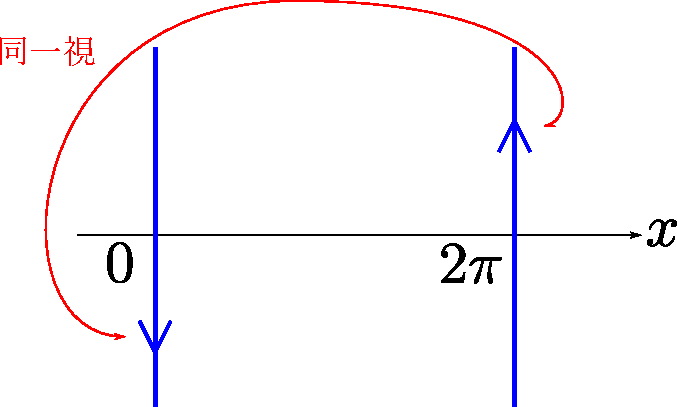
\includegraphics{spinor1d.pdf}
  \caption{$S^1$上のスピノール束$S$。$x=0$と$x=2\pi$の部分が反対向きに貼り合わされている。}
  \label{fig:spinor1d}
\end{figure}


もう一つはエルミート直線束$E\to Y$です。この上に$\U(1)$接続$A$をとります。これは、各点ごとに基底を選ぶとベクトル場$A(x)$で表されます。物理では、この接続、あるいはそれを表すベクトル場を\strong{ゲージ場}と呼びます。

本当はフェルミオンの場を考えたいのですが、ひとまずボゾンの場(普通の関数みたいなもの)
\begin{align}
  \phi\in \Gamma(S\otimes E),\quad \phib \in \Gamma((S\otimes E)^{*})
\end{align}
を考えます。$E$の基底をとると局所的に関数に書けます。これを$\phi(x),\phib(x)$と書きます。$S$の効果は境界条件
\begin{align}
  \phi(x+2\pi)=-\phi(x),\quad \phib(x+2\pi)=-\phib(x)\label{NSBC}
\end{align}
を課すことで取り入れることにします。

これを踏まえて、$\phi(x)$と同じラベルを持つフェルミオン(Grassmann代数の生成子)を$\psi(x)$、$\phib(x)$と同じラベルを持つフェルミオンを$\psib(x)$とします。これら$\psi(x),\psib(x)$が、今の例での場です。

$\psi(x)$に対する共変微分は
\begin{align}
  D_1\psi(x)=\del_{x}\psi(x)-iA(x)\psi(x)
\end{align}
となります。これを用いて作用は
\begin{align}
  S(\psi,\psib,A)=\int dx \psib(x)iD_1 \psi(x)\label{1daction}
\end{align}
で与えることにします。


\subsection{発散}
今の例で分配関数がどうなるか考えてみましょう。分配関数は、
\begin{align}
  Z(A)=\int D\psib D\psi e^{-S(\psi,\psib,A)}
\end{align}
というものを考えたいわけです。式\eqref{finitefermiondet}を踏まえると
\begin{align}
  Z(A)\text{``}=\det(iD_1)\text{''}
\end{align}
となるような気がします。

詳しく考える前に素朴に分配関数に期待する性質(対称性)について考えてみます。
\begin{enumerate}
  \item $iD_1$はエルミート演算子ですからその行列式である$Z(A)$は実数であると期待します。これを「T対称性」と呼びます。
  \item 今は$E$の基底をとって考えましたが、基底のとり方によらないことを期待します。物理では、この基底の取り替えを「$\U(1)$ゲージ変換」、基底のとり方によらないことを「$\U(1)$ゲージ対称性」と呼びます。
\end{enumerate}

さて$Z(A)$について、もう少し考えてみましょう。行列式ですから、有限次元のときとのアナロジーを考えると、固有値の積で書けていると期待できます。$iD_1$の固有値は数学的にちゃんと定義された概念です。とりあえず、これを求めてみましょう。固有値を$\lambda$として固有値方程式$iD_1\phi=\lambda \phi$を考えていきます。変形すると
\begin{align}
  \del_x\phi=i(A-\lambda)\phi
\end{align}
と書けます。これは簡単に解けて
\begin{align}
  \phi(x)=\exp\qty(i\int_{0}^{x} d\xi(A(\xi)-\lambda))\phi(0)
\end{align}
となります。特に
\begin{align}
  \phi(2\pi)=e^{2\pi i (a-\lambda)}\phi(0),\quad a:=\frac{1}{2\pi}\int_{0}^{2\pi}dx A(x)
\end{align}
となります。境界条件\eqref{NSBC}を考えると$e^{2\pi i(a-\lambda)}=-1$となるので
\begin{align}
  \lambda=r+a,\quad r\in \halfint
\end{align}
と固有値のスペクトルが求まります。ここから、分配関数は
\begin{align}
  Z(A)=\prod_{r\in \halfint} \lambda_{r},\qquad \lambda_r:=r+a
\end{align}
となりそうな気がします。しかしここで固有値の積は発散する無限積ですから、この$Z(A)$の表式は意味を持ちません。これは、はっきりと「困ったこと」です。

この発散の問題に対する我々の対処方法は次のようなものです。カットオフと呼ばれる大きな正の実数$\Lambda$と、$\Lambda$による有限の量$Z_{\Lambda}$を導入します。そして、$Z$を
\begin{align}
  Z=\lim_{\Lambda\to \infty}Z_{\Lambda}\label{continuumlimit}
\end{align}
と定義します。$Z_{\Lambda}$は今考えたい問題をちゃんと表しているように、そして極限が有限であるように決めます。とりあえず$Z_{\Lambda}$を有限にすることを「正則化」、そして$Z$を有限にするために作用$S$を$\Lambda$によってうまく決めることを「繰り込み」と呼びます。

もちろん1つの問題に対して$Z_{\Lambda}$の決め方は何通りもある場合もありますし、存在しない場合もあります。物理では$Z_{\Lambda}$の決め方のことを繰り込みの「スキーム」と呼びます。本当に物理で観測される量はスキームに依存すべきではありません。あるいは、スキームによることが避けられないなら、それらは別の理論とするべきです。

さて、いろいろ難しい問題はあるのですが、ここで考えたい問題は次のものです。
\begin{myquote}
  式\eqref{continuumlimit}で得られる$Z$は、素朴に期待する対称性を持つか?
\end{myquote}
これについて、これから具体的なスキームをとって考えていきます。

その前に$\U(1)$ゲージ対称性について考えておきます。これからとるスキームでは、$Z_{\Lambda}$、そして$Z$は$a$の関数になります。$\U(1)$ゲージ変換で$a$がどのように変わるかを見ておきます。基底の変換は、各点ごとに基底の位相を変えます。$\alpha:Y\to \Rb/2\pi \Zb$として$\psi(x)\to e^{i\alpha(x)}\psi(x)$のような変換を考えた場合、
\begin{align}
  A(x)\to A'(x)=A(x)+\del_{x}\alpha(x)
\end{align}
と変化します。このとき$a$は
\begin{align}
  a'=\frac{1}{2\pi}\int_{0}^{2\pi}dx A'(x)=a+\frac{1}{2\pi}\int_{0}^{2\pi}dx \del_{x}\alpha(x)
\end{align}
と変化します。$\frac{1}{2\pi}\int_{0}^{2\pi}dx \del_{x}\alpha(x)$は$\alpha$の巻き付き数であり、整数値をとります。したがって$Z$が$a$の関数として書ける場合、$\U(1)$ゲージ対称性があるかどうかは
\begin{align}
  Z(a+1)=Z(a)
\end{align}
が成り立っているかどうか、ということになります。


\subsection{運動量カットオフ}
1つめのスキームでは、正則化に「運動量カットオフ」と呼ばれる方法を用います。これは、$\lambda_r,\ (r\in \halfint)$の積を
\begin{align}
  \prod_{r\in \halfint}\lambda_r\ \longrightarrow\ \prod_{r\in \halfint, |r|<\Lambda}\lambda_r
\end{align}
として有限積にするものです。これは$\Lambda\to\infty$で今考えている問題の分配関数になりそうなものですね。

もちろんこのまま極限をとったのでは、発散してしまいますから、次のようなものを考えます。(式が煩雑になるので$r\in\halfint$は書かないことにします。)
\begin{align}
  \Zcut_{\Lambda}:=2\frac{\prod_{|r|<\Lambda}\lambda_r}{\prod_{|r|<\Lambda}r}.\label{momentumcut}
\end{align}
これはもちろん問題を「手で変えて」いるのですが、出鱈目にかえているのではありません。かけた量は$a$によらない量ですから、$a$依存性は「変えていない」はずです。

\eqref{momentumcut}まで来れば、有限積ですから順番の入れ替えなどは自由です。変形していくと
\begin{align}
  \Zcut_{\Lambda}:=
  2\prod_{|r|<\Lambda}\frac{r+a}{r}
  =2\prod_{|r|<\Lambda}\qty(1+\frac{a}{r})
  =2\prod_{0<r<\Lambda}\qty(1+\frac{a}{r})\qty(1-\frac{a}{r})
  =2\prod_{0<r<\Lambda}\qty(1-\frac{a^2}{r^2})
\end{align}
となります。したがって$\cos$の無限積表示を用いると
\begin{align}
  \Zcut=\lim_{\Lambda\to \infty}\Zcut_{\Lambda}=2\cos \pi a\label{cutparitionfunction}
\end{align}
となります。

さて、対称性について考えていきます。まず、T対称性について\eqref{cutparitionfunction}は実数ですから、これは保っています。
一方で、$\U(1)$ゲージ対称性について考えると
\begin{align}
  \Zcut(a+1)=-\Zcut(a)
\end{align}
ですから保っていないことになります。これは、式\eqref{momentumcut}の段階で、あらわには保っていないです。まとめると、今のスキームでは\strong{T対称性は保っているが、U(1)ゲージ対称性は保っていない}ということになります。実はこれはアノマリーの現れです。

ここでちょっと寄り道してアノマリーの解釈について今の例で説明します。今$\Zcut$を$\U(1)$接続全体から実数への関数と思うことは出来なかったわけです。しかし$\Zcut$は、ある$\U(1)$接続全体の空間上のある実直線束の切断だと思うことはできます。今の例では、$\U(1)$接続全体の空間は$e^{2\pi ia}$でパラメータ付けされる$S^1$になります。図\ref{fig:configspace}のように$\Zcut$は、$S^1$上の非自明な実直線束の切断になっています。この直線束が自明でなく非自明であるところが、アノマリーの現れです。
\begin{figure}[htbp]
  \centering
  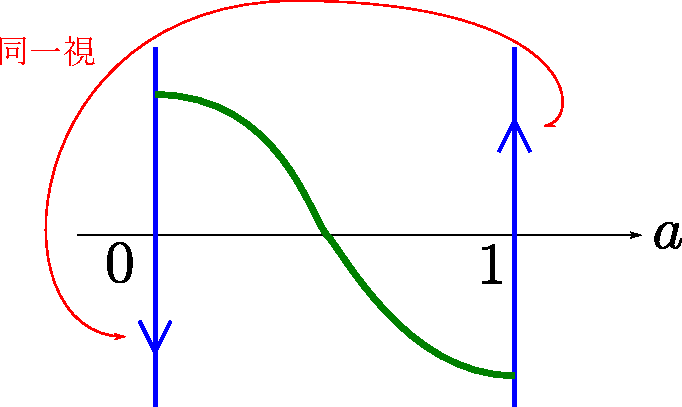
\includegraphics{configspace.pdf}
  \caption{ゲージ場の配位の空間とその上のベクトル束。緑の線で表した分配関数はゲージ場の配位の空間上の関数ではなく、非自明なベクトル束の切断になっている。}
  \label{fig:configspace}
\end{figure}

\subsection{Pauli-Villars正則化}
別のスキームを考えます。正則化はPauli-Villars正則化と呼ばれるものを採用します。

$\lambda_r=0$となる固有値があると分配関数が$0$になるので、問題はなくなります。なのでしばらく$\lambda_r\ne 0,\ (r\in \halfint)$としておきます。

ひとまず、正則化として$\Lambda_1,\Lambda_2,\Lambda_3$を大きな正の実数として
\begin{align}
  \ZPV_{\Lambda}=\Omega \prod_{r\in \halfint}\frac{\lambda_r(\lambda_r+i\Lambda_2)}{(\lambda_r-i\Lambda_1)(\lambda_r+i\Lambda_3)}\label{partitionfunctionPV0}
\end{align}
とします。$\Lambda_1+\Lambda_2-\Lambda_3=0$にすれば、この無限積は絶対収束します。$\Omega$は$a$によらない定数です。
各因子は$\lambda_r\ll \Lambda_1,\Lambda_2,\Lambda_3$の場合に$\lambda_r$の定数倍になりますから、$\Lambda\to 0$で全体にかかる$a$によらない定数を除いて今の問題の分配関数といえるものになっています。そういう意味で今の問題の正則化になっています。

式\eqref{partitionfunctionPV0}は絶対収束しますから、積の順番を自由に入れ替えることができるので、前と同じ計算ができて
\begin{align}
  \ZPV_{\Lambda}=\Omega \frac{\cos\pi a\, \cos \pi(a+i\Lambda_2)}{\cos\pi(a-i\Lambda_1)\cos\pi(a+i\Lambda_3)}
\end{align}
となるので$\Lambda\to \infty$の極限で
\begin{align}
  \ZPV_{\Lambda}
  \to \Omega 2\cos \pi a\frac{e^{-\pi i a+\pi\Lambda_2}}{e^{\pi i a+\pi\Lambda_1}e^{-\pi i a+\pi\Lambda_3}}
 =\Omega e^{-\pi i a} 2 \cos\pi a  e^{\pi(-\Lambda_1+\Lambda_2-\Lambda_3)}
\end{align}
となります。$\Omega=e^{-\pi(-\Lambda_1+\Lambda_2-\Lambda_3)}$とすると
\begin{align}
  \ZPV=\lim_{\Lambda\to \infty}\ZPV_{\Lambda}=2e^{-\pi i a}\cos\pi a
\label{partitionfunctionPV}
\end{align}
となります。

対称性があるかどうかを調べましょう。\eqref{partitionfunctionPV}は一般に複素数ですから、T対称性は破っています。これは、\eqref{partitionfunctionPV0}の$\ZPV_{\Lambda}$の時点であらわには破っています。一方で、
\begin{align}
  \ZPV(a+1)=\ZPV(a)
\end{align}
ですから$\U(1)$ゲージ対称性は保っています。つまり\strong{T対称性は保っていないが、U(1)ゲージ対称性は保っている}ということになります。先程の運動量カットオフとは逆になっていますね。

ここまで見てきた2つのスキームを見てみると、T対称性と$\U(1)$ゲージ対称性を同時に保つことは無理なように思えます。このように素朴に期待する対称性が保てないことを\strong{アノマリー}と呼びます。今の場合T対称性と$\U(1)$ゲージ対称性を同時に保てないので混合アノマリーと呼ばれたりします。

しかし、これは本当でしょうか。今2つのスキームで両方の対称性を保つのは無理ということが分かったのですが、もしかしたら、もっとうまいスキームを持ってくれば両方の対称性をいっぺんに保つことが出来るのではないでしょうか。しかし、すべてのスキームを試してみるのは不可能です。

したがって、アノマリーをもっとよく理解するためには、もう少し見通しの良い見方が必要です。そのような見方の1つが\strong{アノマリー流入}(anomaly inflow)です。

\subsection{η不変量}
アノマリー流入にいく前に、今回重要になる概念の1つであるη不変量を導入します。

$\ZPV$の位相について考えてみましょう。
\begin{align}
  \ZPV=2e^{-i\pi a} \cos \pi a=|\ZPV|e^{i\pi ([a+1/2]-a)}\label{phasePVexplicit}
\end{align}
となります。これはちゃんと正則化して求めた値なので、正しい値です。

この位相をもっと怪しい方法で求めてみます。$\Omega$はある正の定数で
\begin{align}
  \ZPV=\Omega \prod_{r}\frac{\lambda_r(\lambda_r+i\Lambda_2)}{(\lambda_r-i\Lambda_1)(\lambda_r+i\Lambda_3)}
  \to \Omega\prod_{r}\frac{i\lambda_r\Lambda_2}{\Lambda_1\Lambda_3}\quad (\Lambda\to \infty)
\end{align}
という感じです。したがって
\begin{align}
  \ZPV=|\ZPV|\prod_{r}i\sign \lambda_r
\end{align}
となりそうな感じです。ここで
\begin{align}
  i\sign \lambda_r=e^{\frac{\pi}{2}i\sign \lambda_r}
\end{align}
ですから
\begin{align}
  \ZPV=|\ZPV|e^{\frac{\pi}{2}i\sum_{r}\sign \lambda_r}\label{phasePV0}
\end{align}
と書いても良さそうでしょう。

ここに出てきた、固有値の符号の和に名前を付けます。一般的なエルミート演算子を$H$とします。ここから$s\in \Cb$で$\Re s$が十分大きいとして
\begin{align}
  \eta(H,s):=\sum_{\lambda:\ H\text{の固有値}}\frac{\lambda}{|\lambda|^{1+s}}
\end{align}
と定義します。$\eta(H,s)$は$\Re s$が十分大きいところで$s$の正則関数になります。それ以外の領域にも出来る限り解析接続して$\eta(H,s)$を定義します。そして、
\begin{align}
  \eta(H):=\eta(H,0)
\end{align}
と定義し、これを\strong{η不変量}と呼びます。$H$が有限次元の演算子の場合は
\begin{align}
  \eta(H)=\sum_{\lambda:\ H\text{の固有値}}\sign \lambda
\end{align}
となりますから、η不変量は固有値の符号の和を無限次元の演算子にも拡張したものということができます。

η不変量を用いると\eqref{phasePV0}は
\begin{align}
  \ZPV=|\ZPV|e^{\pi i\frac{1}{2}\eta(iD_1)}\label{phasePV1}
\end{align}
と書けると予想できます。

このことに関していくつか注意を述べます。
\begin{itemize}
  \item 式\eqref{phasePV1}の表式には特に$iD_1$の詳細は使っていないので、他の演算子の場合も同様の表式が出来ると予想できます。
  \item $iD_1$のスペクトルは分かっているので、$\eta(iD_1)$は定義にしたがって計算することが出来ます。計算は付録\ref{app:calceta}に書いておきました。結果は$\eta(iD_1)=2[a+1/2]-2a$となり、式\eqref{phasePV1}に代入すると正しい答え\eqref{phasePVexplicit}と一致します。ですから少なくとも今の例に関しては、\eqref{phasePV1}の表式は正しいです。
  \item 一般の場合にも、おそらく\eqref{phasePV1}と同様の表式が正当化されると思います。
  \item この位相は正則化のしかたによっています。例えば\eqref{partitionfunctionPV0}の代わりに、$\Lambda_1$の前の符号を変えて
  \begin{align}
    \ZPV_{\Lambda}=\Omega \prod_{r\in \halfint}\frac{\lambda_r(\lambda_r+i\Lambda_2)}{(\lambda_r+i\Lambda_1)(\lambda_r+i\Lambda_3)}\label{partitionfunctionPV3}
  \end{align}
  とすると
  \begin{align}
    \ZPV=|\ZPV|e^{-\pi i\frac{1}{2}\eta(iD_1)}
  \end{align}
  となります。
  \item \eqref{partitionfunctionPV0}や\eqref{partitionfunctionPV3}の位相を考えるとき、$\Lambda_2$を含む因子と$\Lambda_3$を含む因子は相殺して効きません。ですので、今後はこれらの因子は書かないで、全体にかかる定数$\Omega$も省いて
  \begin{align}
    \ZPV_{\Lambda}=\prod_{r\in \halfint}\frac{\lambda_r}{\lambda_r-i\Lambda}
  \end{align}
  のように略記します。あるいはもっとラフに極限等も略して
  \begin{align}
    \ZPV=\frac{\det(iD_1)}{\det(iD_1-i\Lambda)}
  \end{align}
  というようにも書きます。
\end{itemize}

\subsection{アノマリー流入}\label{subsec:anomalyinflow}
さて、今考えている1次元系の対称性について、これまでの議論では次の2つの選択肢しかなさそうです。
\begin{itemize}
  \item T対称性を諦める。
  \item $\U(1)$ゲージ対称性を諦める。
\end{itemize}
実は、もう1つの選択肢があります。
\begin{itemize}
  \item 1次元の系であることを諦める。
\end{itemize}
これから、これについて説明します。

\begin{figure}[htbp]
  \centering
  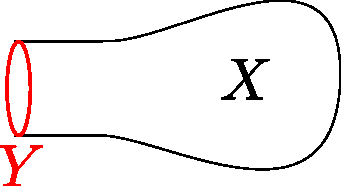
\includegraphics{inflow.pdf}
  \caption{境界が$Y$になっている2次元多様体}
  \label{fig:inflow}
\end{figure}
図\ref{fig:inflow}のように、$X$は2次元Riemann多様体で$\del X=Y$となるようなものとします。この上にエルミート直線束$\Et$とその接続$\At$を$\Et|_{Y}=E,\ \At|_{Y}=A$となるようにとります。$\At$の曲率を$F$とします。パッチをとって、$\At$を1形式$\At$で表わしたとき$F$は2形式で
\begin{align}
  F=d\At
\end{align}
と書けます。$F$は$\U(1)$ゲージ変換で不変です。記号を簡単にするために$(X,\Et,\At)$をまとめて単に$X$と書いておきます\footnote{本当は$S$も$X$に拡張して、これもまとめて単に$X$と書いておきます。}。

$X$を1つ決めたとき、次のような量を定義します。
\begin{align}
  \Zt_{X}:=\ZPV e^{\pi i(\frac{1}{2\pi}\int_{X}F)}
  =|\ZPV|e^{\pi i(\frac{1}{2}\eta(iD_1)+\frac{1}{2\pi}\int_{X}F)}.\label{2dpartitionfunctionwithboundary}
\end{align}
この$\Zt_{X}$は$\U(1)$ゲージ対称性とT対称性の両方を保っていることを説明します。

$\ZPV$と$F$が$\U(1)$ゲージ変換で不変です。なので$\Zt_{X}$も$\U(1)$ゲージ変換で不変で、$\U(1)$ゲージ対称性を保っています。

次にT対称性を見てみます。これは
\begin{align}
  I_{X}:=\frac{1}{2}\eta(iD_1)+\frac{1}{2\pi}\int_{X}F
\end{align}
を見れば良いです。実はAtiya-Patodi-Singer(APS)指数定理から、$I_{X}$が$X$上のある微分演算子の指数であって、整数であることが保証されます。APS指数定理については後に説明します。APS指数定理とは別に、今の場合に$I_{X}$が整数になることを見ておきましょう。$X=D^2$をディスクとして、全体を1つのパッチにとります。この場合、$\At$は1形式とみなすことができて、ストークスの定理を用いて
\begin{align}
  \frac{1}{2\pi}\int_{X} F=\frac{1}{2\pi}\int_{Y}A=a
\end{align}
となります。また$\frac12 \eta(iD_1)=[a+1/2]-a$でしたから
\begin{align}
  I_{D^2}=[a+1/2]-a+a=[a+1/2]
\end{align}
となって、整数になります。一般の$X$の場合には、
\begin{align}
  I_{X}-I_{D^2}=\frac{1}{2\pi} \int_X F-\frac{1}{2\pi} \int_{D^2} F=\frac{1}{2\pi} \int_{X''}F
\end{align}
となります。$X''$は$X$に$D^2$を裏返して$Y$のところで貼り合わせてできる閉じた多様体です。ですから右辺は整数になります。$I_{D^2}$も整数でしたから$I_{X}$も整数です。

このように、$Y$に高い次元の空間$X$を付け加えることによって、対称性をちゃんと保つことができました。このような現象のことを\strong{アノマリー流入}(anomaly inflow)とよびます。$X$から$Y$にアノマリーが流れ込んでいって、$Y$にいたアノマリーと相殺するというイメージです。

アノマリー流入は、アノマリーに対する新しい見方を与えてくれます。歴史的にも、この講義の流れ的にもアノマリーは対称性の非存在ということでした。アノマリー流入を考えると、対称性はいつも存在できます。その代わりに問題は分配関数が付け加える多様体に依存しているということになりました。つまり、アノマリーとは「分配関数$\Zt_X$の付け加える高次元多様体$X$(と構造)への依存性」であると言えます。もし$\Zt_X$が$X$によっていれば、アノマリーはあるし、$\Zt_X$が$X$によっていなければ、アノマリーはありません。

\begin{figure}[htbp]
  \centering
  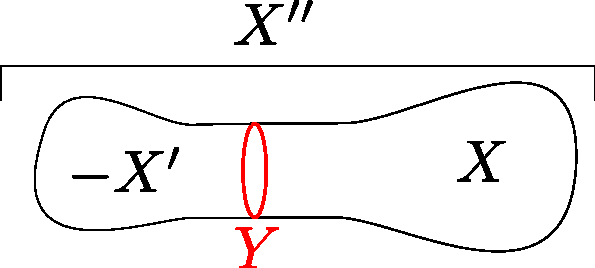
\includegraphics{inflowdifference.pdf}
  \caption{$Y$を境界とする2つの多様体$X,X'$。$X''$は$X$に$X'$を裏返して$Y$のところで貼り合わせたもの。}
  \label{fig:inflowdifference}
\end{figure}
今の例で、$X$への依存性を見てみましょう。$Y$を境界とする多様体$X,X'$をとってきます。
\begin{align}
  \frac{\Zt_{X}}{\Zt_{X'}}=e^{\pi i(I_{X}-I_{X'})}
\end{align}
となります。さらに
\begin{align}
  I_{X}-I_{X'}=\frac{1}{2\pi} \int_X F-\frac{1}{2\pi} \int_{X'} F=\frac{1}{2\pi} \int_{X''}F
\end{align}
となります。$X''$は$X$に$X'$を裏返して$Y$のところで貼り合わせてできる閉じた多様体です。左辺は任意の整数をとりますので、$\Zt_{X}\ne \Zt_{X'}$となることがありえます。したがって、今の例にはアノマリーがあります。

別の例を考えましょう。今の例のコピーを$N_f$個持ってきたものを考えます。$\psi_i(x),\psib_i(x),\ (i=1,2,\cdots,N_f)$として、作用を
\begin{align}
  S=\int dx \sum_{i=1}^{N_f}\psib_i(x) iD_1 \psi_i(x)
\end{align}
とします。同じようにPV正則化をすると
\begin{align}
  \ZPV=|\ZPV|e^{\pi i(N_f \frac12\eta(iD_1))}
\end{align}
となります。この場合、$\Zt_X$は
\begin{align}
  \Zt_X=\ZPV e^{\pi i \frac{N_f}{2\pi}\int_X F}
  =|\ZPV|e^{\pi i(N_f \frac12\eta(iD_1)+\frac{N_f}{2\pi}\int_X F)}
\end{align}
となります。$X$依存性は
\begin{align}
  \frac{\Zt_{X}}{\Zt_{X'}}=e^{\pi i N_f \frac{1}{2\pi}\int_{X''}F}
\end{align}
となります。したがって$N_f$が奇数のときはアノマリーがあり、$N_f$が偶数のときはアノマリーがないことになります。

さて、これから考えたいのは
\begin{myquote}
  $\Zt_{X}$は一体何か?
\end{myquote}  
ということです。さきほどは天下り的に与えて、対称性を保っていることを見ました。では、これに対する2次元の場の理論はあるのでしょうか。これは、物性物理での最近の発展である\strong{SPT相}(symmetry protected topological phase, 対称性で守られたトポロジカル相)になっているということが言われています。この後は、このSPT相から、どのようにして$\Zt_{X}$が出てくるか、そしてAPS指数定理がどうして絡んでくるかについてお話していきたいと思います。

\section{スピノール}
準備として、スピノールの簡単な導入をします。

\subsection{Clifford代数}
まず、Clifford代数を導入します。$n>0$を整数として$\gamma^{a}\ (a=1,\dots,n)$という記号を導入します。$\gamma^a$から生成される自由代数に関係式
\begin{align}
  (\gamma^a)^2=1,\quad \gamma^a\gamma^b=-\gamma^b\gamma^a
\end{align}
を入れたものを\strong{Clifford代数}と呼びます。

Clifford代数の既約表現の同値類は$n$が偶数のときには1種類のみ、$n$が奇数のときには、2種類あります。これらの次元は$2^{[n/2]}$次元です。これから、この表現行列のことを単に$\gamma^{a}$と書くことにします。$\gamma^a$はエルミート行列にとっておきます。

Clifford代数が物理で重要になる理由は、Lie代数$\so(n)$をその部分集合として含んでいることです。記号$\gamma^{ab}$を
\begin{align}
  \gamma^{ab}:=\frac12 [\gamma^{a},\gamma^{b}]
\end{align}
として導入します。これから生成されるベクトル空間
\begin{align}
  \spin(n)=\oplus_{a<b}\Rb \gamma^{ab}
\end{align}
を考えると、これが交換関係で閉じていて、Lie代数をなします。これをよく見てやるとLie代数として$\spin(n)$と$\so(n)$は同型になります。

$\spin(n)$の$\exp$からできるLie群を考えましょう。これを
\begin{align}
  \Spin(n):=\qty{\exp(\sum_{a<b}\omega_{ab}\gamma^{ab})\Bigg| \omega_{ab}\in \Rb}
\end{align}
と定義します。$\Spin(n)$は単連結のLie群になっています。$\Spin(n)$は$\SO(n)$の二重被覆になっています。つまり群の準同型
\begin{align}
  \rho:\Spin(n)\to \SO(n)
\end{align}
があって、$2:1$の写像になっています。

$n$が偶数の場合、すべての$\gamma^a$と反交換する元があります。これを
$n=2k$として
\begin{align}
  \gammab:=(-i)^{k}\gamma^{1}\cdots \gamma^{n}
\end{align}
と書きます。これは$\gammab^2=1$を満たし、$\tr \gammab=0$ですから$\gammab$の固有値は$\pm 1$で、それぞれ$2^{\frac{n}{2}-1}$重縮退になります。また、$\gammab$はエルミート行列です。
$[\gammab,\gamma^{ab}]=0$ですから、Clifford代数の$2^k$次元の表現から導かれる$\so(2k)$の表現は既約ではありません。この表現は$\gammab$の固有値が$+1$の既約表現と$-1$の既約表現の直和に分解されます。これらの$\so(2k)$既約表現は\strong{Weylスピノール}と呼ばれます。また$\gammab$の固有値は\strong{カイラリティ}と呼ばれます。

\subsection{スピン構造}
ここでは、空間の上でのスピノール場を考えたいので、スピノール束と呼ばれるベクトル束を導入します。これは、接ベクトル束から決まる主$\SO(n)$束を「持ち上げて」できる主$\Spin(n)$束を考えることにより、作ることができます。

$X$を$n$次元の向きのついたRiemann多様体とします。$X$を可縮なパッチに分け、1つのパッチの上で座標$x^{\mu}\ (\mu=1,\dots,n)$をとります。計量を
\begin{align}
  ds^2=g_{\mu\nu}(x)dx^{\mu}dx^{\nu}
\end{align}
とします。1つの項に同じ添字が2回現れるとその添字について和をとるというEinsteinの規約を用いています。

余接ベクトル束$T^{*}X$を考えます。このパッチの中の各点ごとに正規直交基底$e^{a}(x)=e^{a}_{\mu}(x)dx^{\mu}$を1つとります。つまり
\begin{align}
  g^{\mu\nu}(x)e^{a}_{\mu}(x)e^{b}_{\nu}(x)=\delta_{ab}
\end{align}
となるようにとります。$g^{\mu\nu}$は$g_{\mu\nu}$の逆行列です。別の言い方をすると$g_{\mu\nu}$が
\begin{align}
  g_{\mu\nu}(x)=\delta_{ab}e^{a}_{\mu}(x)e^{b}_{\nu}(x)
\end{align}
と書けます。なので$e^{\mu}_{a}=g^{\mu\nu}\delta_{ab}e^{b}_{\nu}$として$e_{a}^{\mu}\del_{\mu}$が接ベクトル束の各点での正規直交基底になります。物理では$e^{a}$のことを\strong{多脚場}(vielbein)と呼んでいます。

接ベクトル束の計量を保つような接続を考えます。特にここではLevi-Civita接続をとっておきます\footnote{問題を具体的にするためにLevi-Civita接続をとっていますが、計量を保つものであれば別のものでもよいです。}。今とった基底でのこの接続の表示を$\omega_{\mu}{}^{a}{}_{b}$と書きます。$a,b$の添字は$\delta_{ab},\delta^{ab}$で上げ下げするので上に書いても下に書いても同じです。つまり$V^a(x)$をベクトル場の成分とすると共変微分は
\begin{align}
  (D_{\mu}V)^a=\del_{\mu}V^{a}+\omega_{\mu}{}^{a}{}_{b}V^b
\end{align}
となります。この$\omega_{\mu}{}^{a}{}_{b}$のことを物理では\strong{スピン接続}と呼んでいます。

スピノール束を考えていきます。1つのパッチ$U_{\alpha}$の上で$S|_{U_{\alpha}}=U_{\alpha}\times \Cb^{m},\ m=2^{[n/2]}$です。この1つの切断を$\psi(x)$としたとき、共変微分は$\omega_{\mu}{}^{a}{}_{b}$をスピノール表現で表したもの
\begin{align}
  D_{\mu}\psi=\del_{\mu}\psi+\frac14\omega_{\mu}{}^{ab}\gamma_{ab}\psi
\end{align}
となります。

次にパッチの貼り合わせを考えます。接ベクトル束の貼り合わせの関数は与えられています。つまり、$U_{\alpha}\cap U_{\beta}\ne \emptyset$の各点$x$で$h_{\alpha\beta}(x)\in \SO(n)$が与えられています。これに対して
$\htl_{\alpha\beta}(x)\in \Spin(n)$を$\rho(\htl_{\alpha\beta}(x))=h_{\alpha\beta}(x)$となるように、そして3つのパッチが重なる部分でちゃんと貼り合うように選びます。このように貼り合わせて出来るベクトル束を\strong{スピノール束}と呼びます。

スピノール束は存在しない場合もあります。また、存在する場合でも、一般には一意ではありません。スピノール束から決まる主$\Spin(n)$束をスピン構造と呼びます。

\subsection{Dirac演算子}\label{subsec:spinorsetup}
$X$をスピン構造付きのRiemann多様体とし、$S\to X$をそのスピノール束とします。$G$をコンパクトLie群とし、$E\to X$を$G$を構造群に持つベクトル束とします。また、$E$の接続を$A$とします。パッチとその中での基底を1つとり、そこでの$\psi(x)\in \Gamma(S\otimes E)$の共変微分を
\begin{align}
  D_{\mu}\psi(x)=\del_{\mu}\psi+\frac14\omega_{\mu}{}^{ab}\gamma_{ab}\psi-iA_{\mu}\psi
\end{align}
とします。$A_{\mu}$は接続$A$を今の基底で行列に値を持つベクトル場で表したものです。これを用いて、$\Gamma(S\otimes E)$上のDirac演算子$D$を
\begin{align}
  D\psi:=\gamma^{\mu}D_{\mu}\psi,\qquad \gamma^{\mu}:=e^{\mu}_{a}\gamma^{a}
\end{align}
と定義します。今はパッチごとに座標と基底をとって定義しましたが、最終的に出来た$D$は座標や基底のとり方によりません。また、$D$は反エルミート演算子になります。

前に述べたように$n$が偶数の場合、すべての$\gamma^a$と反交換する$\gammab$が存在します。この場合$\gammab$も$\Gamma(S\otimes E)$に作用していて
\begin{align}
  \gammab D=-D\gammab
\end{align}
という関係を満たします。

\section{2次元のフェルミオン}\label{sec:massless}
第\ref{1dfermion}節で紹介したアノマリーを2次元の立場から理解するために、ここでは2次元の場合に指数定理を紹介します。

\subsection{場と作用}\label{subsec:2dsetup}
$X$を2次元スピン構造付きのRiemann多様体とし、$S\to X$をそのスピノール束$E\to X$をエルミート直線束、$E$の$\U(1)$接続を$A$とします。$\psi(x),\psib(x)$を$\Gamma(S\otimes E),\Gamma((S\otimes E)^{*})$の元をフェルミオンにした場とします。作用を
\begin{align}
  S=\int_{X}d^2x\sqrt{g}\psib iD \psi
  \label{2dmasslessaction}
\end{align}
とします。

この理論での期待値を考えます。$F(\psi,\psib)$を$\psi,\psib$のゲージ不変な汎関数として
\begin{align}
  \expval{F}:=\int D\psib D\psi F(\psi,\psib) e^{-S}
  \label{2dmasslessexpval}
\end{align}
とします。実は分配関数を考えると$0$になることがあるので規格化は深く考えないことにします。

\subsection{Atiyah-Singer指数定理}
先程の設定で、$X$が閉じた多様体の場合を考えます。このとき、Atiyah-Singer(AS)の指数定理を、軸性$\U(1)$アノマリーと呼ばれるアノマリーの立場から説明したいと思います。

\eqref{2dmasslessaction}を見ると、$\alpha$を実数の定数として変換
\begin{align}
  \psi\to \psi'=e^{i\alpha \gammab}\psi,\qquad \psib\to\psib'=\psib e^{i\alpha\gammab}\label{axialu1transf}
\end{align}
で$S$は不変であることが分かります。この変換を軸性$\U(1)$変換と呼んでおきましょう。

積分測度$D\psib D\psi$は軸性$\U(1)$変換でどうなるでしょうか?素朴には、頑張ってうまいスキームをとってくれば、この測度も軸性$\U(1)$変換で不変になるようにできると期待できます。しかし、$\U(1)$ゲージ対称性を保つ限り、この軸性$\U(1)$対称性を保つようなスキームはないということが知られています。これは\strong{軸性U(1)アノマリー}と呼ばれ、Adler\cite{Adler:1969gk}と Bell, Jakiw\cite{Bell:1969ts}によって発見されました。ですので、軸性$\U(1)$アノマリーはABJアノマリーとも呼ばれます。今のような経路積分の見方と、それを用いた計算方法は藤川\cite{Fujikawa:1979ay}によって開発されました。

軸性U(1)アノマリーがあっても、これの性質を知っていれば、系を調べるのに役に立ちます。$\psi,\psib$によらない``Jacobian''$J$で
\begin{align}
  D\psib' D\psi'=D\psib D\psi J\label{Jacobian}
\end{align}
となったと仮定します。そうすると次のようにして\eqref{2dmasslessexpval}で表される期待値の間に関係式が得られ、この系の性質に関する情報が得られます。まず、期待値の定義\eqref{2dmasslessexpval}に当てはめて、積分変数を$\psi,\psib$から$\psi',\psib'$に書き換えて計算していきます。すると
\begin{align}
  \expval{F(\psi,\psib)}
  &=\int D\psib D\psi F(\psi,\psib) e^{-S(\psi,\psib)}
  =\int D\psib' D\psi' F(\psi',\psib') e^{-S(\psi',\psib')}\nonumber\\
  &=J\int D\psib D\psi F(\psi',\psib') e^{-S(\psi,\psib)}
  =J\expval{F(\psi',\psib')}
\end{align}
という関係式が得られます。

では、$J$がどうなるかを調べましょう。このためにエルミート演算子$D^2$の固有値問題を考えます。これは数学的にちゃんと定義された問題です。まず、カイラリティの演算子$\gammab=-i\gamma_1\gamma_2$が$\gamma_a$と反交換することを思い出すと
\begin{align}
  \gammab D=-D\gammab,\quad \gammab D^2=D^2\gammab
\end{align}
となるので、$D^2$と$\gammab$は同時対角化できます。$D^2$は半負定値です。まず固有値を$-\lambda_n^2<0$として、対応する固有ベクトルがカイラリティが$+$で$u_{+n}$であったとします。
\begin{align}
  D^2u_{+n}=-\lambda_{n}^2u_{+n},\quad \gammab u_{+n}=+u_{+n}.
\end{align}
このとき、$u_{-n}:=\frac{1}{\lambda_n}Du_{+n}$とすると
\begin{align}
  D^2u_{-n}=-\lambda_{n}^2u_{-n},\quad \gammab u_{-n}=-u_{-n}.  
\end{align}
となります。つまり、$D^2$の$0$でない固有値に対応する固有ベクトルは必ずカイラリティ$+$のものとカイラリティ$-$のものがペアで現れるということです。$0$固有値はペアになっているとは限りません。$0$固有値に対応するカイラリティ$\pm$の固有ベクトルをそれぞれ
\begin{align}
  w_{+i}\ (i=1,\dots,n_+),\quad w_{-i}\ (i=1,\dots,n_-)
\end{align}
としておきます。

これを踏まえて、$\psi,\psib$を$u_{\pm n},w_{\pm i}$で展開します。正則化のために$n$の和は$\lambda_{n}^2<\Lambda^2$の範囲内だけでとることにします。
\begin{align}
  \psi=\sum_{n}(c_{+n}u_{+n}+c_{-n}u_{-n})
  +\sum_{i=1}^{n_+}b_{+i}w_{+i}
  +\sum_{i=1}^{n_-}b_{-i}w_{-i},\nonumber\\
  \psib=\sum_{n}(\cb_{+n}u_{+n}^{\dag}+\cb_{-n}u_{-n}^{\dag})
  +\sum_{i=1}^{n_+}\bb_{+i}w_{+i}^{\dag}
  +\sum_{i=1}^{n_-}\bb_{-i}w_{-i}^{\dag}.
\end{align}
$c_{\pm n},\cb_{\pm n}, b_{\pm i},\bb_{\pm i}$はフェルミオン(Grassmann代数の生成子)であることに注意してください。こうしておくと正則化された積分測度$D\psib D\psi$は$\Omega$を定数として
\begin{align}
  D\psib D\psi=\Omega \prod_{n}(d\cb_{+n}d c_{+n}d\cb_{-n}d c_{-n})\prod_{i=1}^{n_+}(d\bb_{+i}db_{+i})\prod_{i=1}^{n_+}(d\bb_{-i}db_{-i})\label{modeintegralmeasure}
\end{align}
とすることができそうです。この正則化は$\U(1)$ゲージ対称性を保ちます。

積分測度\eqref{modeintegralmeasure}の軸性$\U(1)$変換を考えてみましょう。$c_{\pm n},\cb_{\pm n}, b_{\pm i},\bb_{\pm i}$に対する軸性$\U(1)$変換は
\begin{align}
  c'_{+n}=e^{i\alpha}c_{+n},\qquad \cb'_{+n}=e^{i\alpha}\cb_{+n},\qquad
  b'_{+n}=e^{i\alpha}b_{+n},\qquad \bb'_{+n}=e^{i\alpha}\bb_{+n},\nonumber\\  
  c'_{-n}=e^{-i\alpha}c_{-n},\qquad \cb'_{-n}=e^{-i\alpha}\cb_{-n},\qquad
  b'_{-n}=e^{-i\alpha}b_{-n},\qquad \bb'_{-n}=e^{-i\alpha}\bb_{-n}
\end{align}
となります。ですから、積分測度\eqref{modeintegralmeasure}のうち、非0モード$c,\cb$の部分は明らかに不変になります。ですから、0モードの部分$b,\bb$のところだけを考えれば良いです。フェルミオンの積分は実は微分だということに注意すると
\begin{align}
  D\psib' D\psi'=D\psib D\psi e^{-2i\alpha(n_{+}-n_{-})}\label{Jacobian2}
\end{align}
を得ます。ですから$J=e^{-2i\alpha(n_{+}-n_{-})}$となることが分かりました。

このJacobianにでてくる$n_{+}-n_{-}$をDirac演算子の\strong{指数}と呼び
\begin{align}
  \Ind(D):=n_{+}-n_{-}\label{defindex}
\end{align}
と書くことにします。実はこの指数が$\U(1)$ゲージ場の曲率$F$を用いて
\begin{important}
  \begin{align}
    \Ind(D)=\frac{1}{2\pi}\int_{X}F
  \end{align}
\end{important}
と書けることが\strong{Atiyah-Singerの指数定理}\cite{Atiyah:1963zz,Atiyah:1968mp}から知られています。ですから
\begin{align}
  J=e^{-2i\alpha \frac{1}{2\pi}\int_{X}F}
\end{align}
となります。この結果は物理の計算\cite{Adler:1969gk,Bell:1969ts,Fujikawa:1979ay}からも知られていました。


\subsection{Atiyah-Patodi-Singer指数定理}
今回問題にしたい指数定理は境界のある多様体の場合の指数定理です。ここでは境界のある多様体上のフェルミオンについて考えてみましょう。

$X$を境界があるコンパクトRiemann多様体とし、$Y=\del X$とします。境界がある場合、境界条件をどうするかというのが問題になります。物理でよく使われる境界条件は、$Y$上での単位法線ベクトルを$n_{a}$として、$Y$上で
\begin{align}
  n_{a}\gamma^{a}\psi=\psi
\end{align}
あるいは
\begin{align}
  n_{a}\gamma^{a}\psi=-\psi
\end{align}
というものです。これは、理論の局所性やユニタリー性などの物理で必要な条件を満たします。しかし、この境界条件は$\gammab$と反交換します。ですから、この系はアノマリーを考える以前に軸性$\U(1)$対称性を持ちません。
指数定理の立場から言うと、この境界条件の元で$D\psi=0$の解は決まったカイラリティを持ちません。したがって、指数は定義できません。

\begin{figure}[htbp]
  \centering
  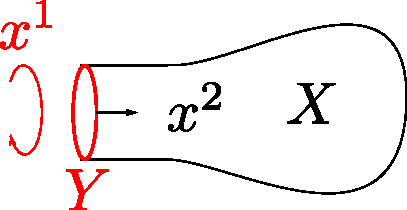
\includegraphics{APSbdy.pdf}
  \caption{境界のある多様体$X$と境界付近での座標のとり方。}
  \label{fig:APSbdy}
\end{figure}
Atiyah, Patodi, Singer\cite{Atiyah:1975jf,Atiyah:1976jg,Atiyah:1980jh}は、次のようなカイラリティを保つ境界条件を考え、そこで指数定理を考えました。この境界条件はAPS境界条件と呼ばれます。図\ref{fig:APSbdy}のように境界のところを少しだけ円筒状に伸ばして、境界の近くで曲率が$0$になるようにします。$Y$の近くで、$Y$に沿った座標を$x^1$、$Y$に垂直な座標を$x^2\ge 0$とし$x^2=0$が$Y$だとします。接ベクトル束の正規直交基底$e^a_{\mu}=\delta^{a}_{\mu}$と選んで$\omega_{\mu}{}^{a}{}_{b}=0$とします。また$E$の基底をうまく選んで$A_2=0$とします。このとき、この付近でのDirac方程式$D\psi=0$は
\begin{align}
  \del_{2}\psi=B\psi,\quad B=-\gamma^{2}\gamma^{1}D_{1}
  \label{0modewithbdy}
\end{align}
となります。$B$はエルミート演算子です。簡単のために$B$は$0$固有値を持たないとします。APS境界条件は、$Y$で
\begin{align}
  \frac{B}{|B|}\psi=+\psi\label{2dAPSbc}
\end{align}
を要求します。\eqref{0modewithbdy}を$Y$から$X$の内側に解いていったとき、指数関数的に増大する方のモードのみを残すということです。$[B,\gammab]=0$ですから、APS境界条件は軸性$\U(1)$アノマリーを保ちます。また、Dirac方程式\eqref{0modewithbdy}の解は決まったカイラリティを持ちますから、指数を定義できます。このAPS境界条件を課したDirac演算子を$\DAPS$と書いておきます。

APS指数定理は、この$\DAPS$の指数に関する定理で、次のように表されます。
\begin{align}
  \Ind(\DAPS)=\frac12 \eta(iD_1)+\frac{1}{2\pi}\int_{X}F.\label{2dAPSindextheorem}
\end{align}
これが\ref{subsec:anomalyinflow}項で出てきたものです。証明はここではやりません。


\begin{figure}[htbp]
  \centering
  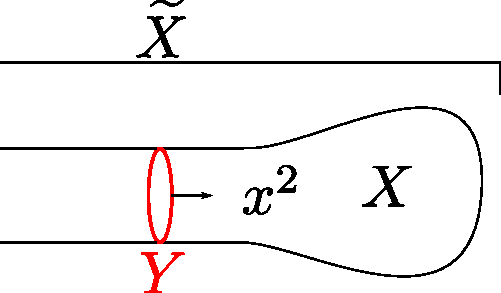
\includegraphics{APSbdyinfinite.pdf}
  \caption{$X$に無限に長い円筒を付け加えて出来る多様体$\widetilde{X}$。}
  \label{fig:APSbdyinfinite}
\end{figure}
境界を入れる代わりに、$X$の境界$Y$に無限に長い円筒$Y\times \Rb_{\le 0}$を付け加えて出来る多様体$\widetilde{X}$を考えることでもAPS指数定理を考えることができます(図\ref{fig:APSbdyinfinite})。$\widetilde{X}$上で$L^2$ノルムが有限な$D\psi=0$の解の個数から決まる指数を考えたとき式\eqref{2dAPSindextheorem}が成り立ちます。これは先程APS境界条件を考えるときにとった座標を用いて考えると理解できます。\eqref{2dAPSbc}の境界条件を満たす\eqref{0modewithbdy}の解を考えると、$x^{2}<0$の方に伸ばしていくことができて、指数関数的に減衰することになり、規格化可能になります。

さて、問題にしたいのは
\begin{myquote}
  なぜ\ref{1dfermion}節で取り扱った1次元の系が、APS指数と関係があるのか。
\end{myquote}
ということです。今までの話では、一応境界が1次元というところは関係がありそうです。しかし、この節で扱った作用\eqref{2dmasslessaction}で表されるような「質量がない」フェルミオンは本当に2次元にあるフェルミオンです。ですから物理としては、このフェルミオンは\ref{1dfermion}節で扱った系とは関係がありません。

\ref{1dfermion}節の系と関係がある2次元の理論を作るためには、フェルミオンに質量を与えて2次元にあるフェルミオンを実質的に「殺す」必要があります。その上で境界のみに質量のないフェルミオンが不可避に現れるようにすれば、ほとんど\ref{1dfermion}で扱った系になります。その2次元の理論の分配関数が\eqref{2dpartitionfunctionwithboundary}の$\Zt_X$になるという主張です。

ということで、質量のあるフェルミオンと指数定理について次節で扱っていきます。


\section{2次元のdomain-wallフェルミオンとAPS指数}
\subsection{質量}
ここでは質量について説明します。大雑把にいうと、質量を今考えているスケールより十分大きくすると、「何もない、空っぽの理論」になってしまうということです。

質量$M$を入れたフェルミオンの作用は、次のようなものです。
\begin{align}
  S=\int_{X}d^2 x \sqrt{g}\psib (iD-iM)\psi.\label{2dmassivefermion}
\end{align}

例えば、この作用で表される系の分配関数を考えるとPauli-Villars正則化をして
\begin{align}
  Z=\frac{\det(iD-iM)}{\det(iD-i\Lambda)}
\end{align}
となります。$\lambda$を$iD$の固有値として
\begin{align}
  Z=\prod_{\lambda}\frac{\lambda-iM}{\lambda-i\Lambda}
\end{align}
となります。$\Lambda$は十分大きいとして、$|\lambda|\ll |M|$のときの因子は
単に$\frac{M}{\Lambda}$となってしまって、多様体の情報とかゲージ場の情報とかが一見消えてしまっています。これが、「空っぽの理論」と呼んでいる1つの理由です。

もう少し、感じをつかむために、フェルミオンの2点相関関数を考えてみます。\eqref{fermion2pt}をそのまま用いると
\begin{align}
  \expval{\psi(x)\psib(x')}=\bra{x}\frac{1}{iD-iM}\ket{x'}
\end{align}
となります。記号の意味は、$x,x'$を固定すると左辺は縦ベクトルと横ベクトルの積ですから正方行列になります。右辺は演算子の逆を考えて、その積分核を表したものです。$X=\Rb^2$でゲージ場が$0$のとき、これは厳密に計算できます。その振る舞いは$|x-x'|\gg 1/|M|$のとき
\begin{align}
  \expval{\psi(x)\psib(x')}\sim e^{-|M||x-x'|}
\end{align}
となり、$1/|M|$より距離が大きくなると急速に小さくなります。一般の$X$の場合にも、$1/|M|$が$X$の曲率やゲージ場のスケールより十分小さかったとすると、その非常に小さい部分では$\Rb^2$と同様になります。まとめると、この2点相関関数は$1/|M|$より十分大きい距離だけ離すと$0$になります。また今の系の相関関数はWickの定理によって2点相関関数の積に書けるので、$1/|M|$より十分大きい距離のスケールを考える限り、すべての相関関数が$0$になります。この意味で今の理論は「空っぽの理論」です。

もう少し具体的にするために、電子を考えてみます。電子は電荷を持っている粒子のうち、もっとも軽いものです。電子の$1/|M|$で表される距離(コンプトン波長と呼ばれます)は約$2.4\times 10^{-12}$mになります。これは、典型的な原子の大きさの1/100くらいです。これより大きなスケールの物理を考える場合、真空中で電子の場があることは無視してよくなります。逆にこれより小さいスケールの物理を考える場合には\footnote{あるいは、非常に精密な測定ができる場合にも考えないとだめです。}、この電子の効果を考える必要があります。

ここで、質量のあるフェルミオンの理論は「空っぽの理論」だと言いました。実は「空っぽの理論」と言いながら、微妙に何か残っているものがあり、それがこれからの議論で重要な役割を果たします。例えば今の場合、$M>0$で大きい場合と$M<0$で絶対値が大きい場合では、両方とも「空っぽの理論」ですが、微妙に「異なる」空っぽの理論です。このような違いを「異なるSPT相にある」という言い方をします。今回、この質量の符号に関するSPT相とDirac演算子の指数の関連について、これから説明していきたいと思います。

\subsection{質量のあるフェルミオンとAS指数}\label{subsec:massiveASindex}
ここでは、質量のあるフェルミオンの理論とAS指数について説明します。ここからは、あまり標準的なお話ではなくて、教科書とかには載っていないお話になります。

$X$を閉じた2次元リーマン多様体とし、ベクトル束などは\ref{subsec:2dsetup}項のものをとります。ただし、作用は質量のあるフェルミオンの作用\eqref{2dmassivefermion}を考えます。ここから、分配関数を作ります。これは、$X$(計量やスピン構造や接続もまとめて$X$と書いておきます)と質量$M$によっているので
\begin{align}
  Z(X,M)=\int D\psib D\psi e^{-S}=\frac{\det(iD-iM)}{\det(iD-i\Lambda)}
\end{align}
と書いておきます。ここでも、Pauli-Villars 正則化を用いていて、簡略化した記号で書いています。質量の符号による違いを考えたいので$M>0$として
\begin{align}
  \frac{Z(X,-M)}{Z(X,M)}=\frac{\det(iD+iM)}{\det(iD-iM)}\label{partitionfunctionratio}
\end{align}
という比を考えることにします。

ここでは、2つのやり方で\eqref{partitionfunctionratio}を考えてみましょう。1つめは、軸性$\U(1)$変換を利用する方法です。質量のあるフェルミオンの理論は、軸性$\U(1)$変換で不変ではありません。実際
\begin{align}
  \psib'\psi'=\psib e^{2i\alpha \gammab}\psi
\end{align}
となります。特に$\alpha=\pi/2$とおくと
\begin{align}
  \psib'\psi'=-\psib \psi
\end{align}
となります。したがって\eqref{2dmassivefermion}の作用を$S(\psi,\psib,M)$と書くと
\begin{align}
  S(\psi',\psib',M)=S(\psi,\psib,-M)
\end{align}
となります。\eqref{Jacobian2}, \eqref{defindex}で$\alpha=\pi/2$とおくと
\begin{align}
  D\psib'D\psi'=D\psib D\psi\, e^{-\pi i \Ind(D)}
\end{align}
となります。したがって
\begin{align}
  Z(X,M)
  =\int D\psib D\psi e^{-S(\psi,\psib,M)}
  =\int D\psib' D\psi' e^{-S(\psi',\psib',M)}
  =e^{-\pi i \Ind(D)}\int D\psib D\psi e^{-S(\psi,\psib,-M)}
\end{align}
となり
\begin{align}
  \frac{Z(X,-M)}{Z(X,M)}=e^{\pi i \Ind(D)}\label{massivephase1}
\end{align}
を得ます。

2つめの説明をします。このために\eqref{partitionfunctionratio}を変形していきます。
\begin{align}
  \frac{Z(X,-M)}{Z(X,M)}=\frac{\det(iD+iM)}{\det(iD-iM)}
  =\frac{\det(i\gammab(D+M))}{\det(i\gammab(D-M))}
\end{align}
となります。ここから少し怪しい変形をしていきます。このために
\begin{align}
  \Hm:=\gammab(D+M)
\end{align}
について考えます。これはエルミート演算子であることに注意します。ですからその行列式は固有値の積で書けて
\begin{align}
  \det(i\Hm)
  =\prod_{\lambda:\text{固有値}}i\lambda
  =\prod_{\lambda:\text{固有値}}|\lambda|e^{i\frac{\pi}{2} \sign \lambda}
  =|\det(i\Hm)|e^{\frac{\pi}{2}i\eta(\Hm)}
\end{align}
となります。ここで固有値の符号の和をゼータ関数正則化で考えたη不変量が出てきます。$\Hp:=\gammab(D-M)$として、
\begin{align}
  \frac{Z(X,-M)}{Z(X,M)}=\qty|\frac{Z(X,-M)}{Z(X,M)}|e^{\pi i \frac12(\eta(\Hm)-\eta(\Hp))}\label{massivephase2}
\end{align}
となります。

\eqref{massivephase1}と\eqref{massivephase2}を比較すると
\begin{align}
  \frac12 \eta(\Hm)-\frac12 \eta(\Hp)\equiv \Ind(D)\mod 2
\end{align}
という結果が得られます。実は、これよりもっと強い関係
\begin{important}
  \begin{align}
    \frac12 \eta(\Hm)-\frac12 \eta(\Hp)=\Ind(D)\label{massiveASindex}
  \end{align}    
\end{important}
が成り立ちます。これが、説明したかった質量のあるフェルミオンとAS指数の関係です。

\eqref{massiveASindex}の1つの証明は\cite{Fukaya:2019qlf}でも書いています。ここでは、別の初等的な証明を紹介します。これには$\Hm$と$D$が反交換することを用います。
\begin{align}
  D\Hm=-\Hm D.
\end{align}
ですから、$\phi$を$\Hm$の固有値$\lambda$の固有ベクトルとし、$D\phi\ne 0$である場合には、
\begin{align}
  \Hm D\phi=-\lambda D\phi
\end{align}
となるので固有ベクトル$D\phi$の固有値が$-\lambda$ということになります。つまり$D\phi\ne 0$のとき、$+\lambda$の固有値と$-\lambda$の固有値が1対1対応しているということです。したがって、$\Re s$が十分大きいとして
\begin{align}
  \eta(\Hm,s):=\sum_{(\lambda,\phi):\Hm\text{の固有値固有ベクトル}}\frac{\lambda}{|\lambda|^{1+s}}
  =\sum_{(\lambda,\phi):\Hm\text{の固有値固有ベクトル},\ D\phi=0}
  \frac{\lambda}{|\lambda|^{1+s}}
\end{align}
となります。最後の表式は有限和ですから、解析接続はできているので$s=0$として
\begin{align}
  \eta(\Hm):=\eta(\Hm,0)=\sum_{(\lambda,\phi):\Hm\text{の固有値固有ベクトル},\ D\phi=0}\sign \lambda
\end{align}
となります。後は$D\phi=0$となる空間での$\Hm$の固有値固有ベクトルを考えれば良いことになります。$D\phi=0$のとき
\begin{align}
  \Hm \phi=\gammab(D+M)\phi=M\gammab \phi
\end{align}
となるので、$\Hm$の固有値の符号は$\gammab$の固有値、つまりカイラリティになります。ここから、固有値の符号の和はAS指数そのものになります。
\begin{align}
  \eta(\Hm)=\Ind(D)
\end{align}
という非常にシンプルな関係が成り立ちます。同様の議論をすると
\begin{align}
  \eta(\Hp)=-\Ind(D)
\end{align}
となるので\eqref{massiveASindex}が成り立つことが証明できました。

物理での伝統的なAS指数の説明は、\ref{sec:massless}節で説明したような質量のないフェルミオンと軸性$\U(1)$アノマリーに関係するものでした。しかし、この節で説明したような質量のあるフェルミオンとの関係は、物理における指数の新しい見方と言えます。ここで見たのは分配関数の符号として現れ、SPT相を区別するのに用いることができるということです。実は\eqref{massiveASindex}のように、偶奇だけでなく整数としての指数も質量のあるフェルミオンのη不変量として表すことができる、というのも様々な物理的応用があると期待しています。

\subsection{domain-wallフェルミオン}

これまでの考察を利用して\ref{subsec:anomalyinflow}項で考えたようなアノマリー流入について、$\Zt$は何か、という問題をもう一度よく考えたいです。

状況としては、質量のないフェルミオンが2次元にあると全く異なる状況になるので、2次元では質量のあるフェルミオン、つまり以前に「空っぽの理論」と呼んだものを用います。

ただし、作用\eqref{1daction}で表されるような1次元の質量のないフェルミオンにはいてほしいので、ここではdomain-wallフェルミオンと呼ばれるものを用います\footnote{\cite{Yonekura:2016wuc,Witten:2019bou}では、質量のあるフェルミオンで境界を入れたものを用いられています。}。これは、2つの異なるSPT相にある理論を$Y$を境界にして貼り合わせたものです。このようにすると境界のところに質量のないフェルミオンが現れることが知られています。

\begin{figure}[htbp]
  \centering
  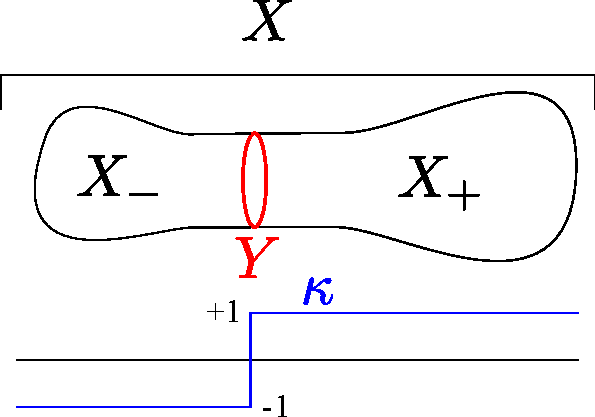
\includegraphics{domainwall.pdf}
  \caption{domain-wallフェルミオンの設定。$X_{+}$と$X_{-}$で別の相にある。それを表すのに$\kappa$という関数を用いている。}
  \label{fig:domainwall}
\end{figure}
設定を詳しく説明します。図\ref{fig:domainwall}を見てください。$X$を閉じた2次元リーマン多様体とし、\ref{sec:massless}で考えたような構造が入っているとします。$X$をその1次元部分多様体$Y$を境界にして2つの部分$X_{+}$と$X_{-}$に分けることにします。ただし、$Y$付近の小さな領域で$Y\times \Rb$と同じになっているとします。関数$\kappa:X\to \Rb$を
\begin{align}
  \kappa(x)=
  \begin{cases}
    -1& x\in X_{-}\\
    +1& x\in X_{+}
  \end{cases}
\end{align}
とします。$Y$上では$\kappa=0$としておきます。$M>0$として、この$X$の上で作用
\begin{align}
  S_{DW}=\int_{X} d^2x\sqrt{g}\psib (iD+iM\kappa(x))\psi
  \label{domainwallaction}
\end{align}
で表されるフェルミオンを考えます。この分配関数はPauli-Villars正則化を考えて
\begin{align}
  &\ZDW=\int D\psib D\psi e^{-S_{DW}}=\frac{\det(i(D+M\kappa))}{\det(i(D-\Lambda))}=\frac{\det(\HDW)}{\det(\HPV)},\nonumber\\
  &\HDW:=\gammab(D+M\kappa),\quad \HPV:=\gammab(D-\Lambda)
  \label{domainwallpartitionfunction}
\end{align}
となります。

\eqref{domainwallaction},\eqref{domainwallpartitionfunction}で表される系には次の性質があります。
\begin{itemize}
  \item $\ZDW$は実数です。これは、$\HDW,\HPV$はエルミート演算子であることから分かります。これは既にちゃんと正則化されたものですから、場の理論特有の微妙さはありません。
  \item $\ZDW$は$\U(1)$ゲージ対称性を保っています。
  \item この系は$Y$に局在化した質量のないフェルミオンがあります。このことは、次に説明するように$\HDW$の$|M|$より絶対値がずっと小さな固有値が$iD_1$の固有値と一致し、固有ベクトルが$Y$付近に局在することから言えます。
\end{itemize}
したがって\ref{subsec:anomalyinflow}項で考えたシナリオに出てくるものとしてふさわしいです。別の言い方をすると
\begin{important}
  domain-wallフェルミオンは\ref{1dfermion}節で考えたフェルミオンのT対称性、$\U(1)$ゲージ対称性は保つが1次元の系の中では閉じていない正則化($M$も$\Lambda$もカットオフとして)である。
\end{important}
と言えます。

さて$\HDW$のスペクトルについて考えましょう。$Y$の付近以外では、質量のあるフェルミオンですから、固有値の絶対値は$|M|$程度以上になります。それよりずっと絶対値が小さい固有値があるとすると、対応する固有ベクトルは$Y$の付近に局在しています。

$|Y|$付近では、$Y\times \Rb$になっています。ここに注目し、具体的に座標をとって考えます。$Y$に垂直に座標$x_2$をとり$x_2=0$が$Y$とし、$x_2>0$が$X_{+}$に入っているとします。$|Y|$に沿って$x_1$をとり、前にやったように$\omega_{\mu}{}^{a}{}_{b}=0,\ A_{2}=0$となるゲージをとります。固有関数を$\phi$、固有値を$\mu$として、固有値方程式は
\begin{align}
  (\gammab\gamma^{2}\del_{2}+\gammab\gamma^{1}D_{1}+M\kappa(x)\gammab-\mu)\phi=0
\end{align}
となります。これは、変数分離可能です。$iD_1$を対角化して$iD_1 u_{\lambda}(x_1)=\lambda u_{\lambda}(x_1)$とし、$\phi=f(x_2)u_{\lambda}(x_1)$とします。$\gammab=-i\gamma^1\gamma^2$であることを考慮すると固有値方程式は
\begin{align}
  f'=(\lambda \gammab - M\kappa(x)\gamma^2+\mu i\gamma^1)f
  \label{tempDWeigeneq}
\end{align}
となります。ここから$\mu=\lambda$であることを示します。

まず、境界条件について説明します。\eqref{tempDWeigeneq}の両辺の$x_2=0$における不連続性について考えます。$f$は連続ですから\footnote{そうでないと$f'$がデルタ関数を含むことになります。}不連続性を比較すると
\begin{align}
  f'(+0)-f'(-0)=-2M \gamma^2 f(0)
\end{align}
となります。今、$Y$から離れると$f$は小さくなるようにしていますから、左辺は負になるはずです。ですから
\begin{align}
  \gamma^2 f(0)=+f(0)\label{tempDWBC}
\end{align}
という境界条件を満たす必要があります。

次に$x_2>0$の領域で\eqref{tempDWeigeneq}を考えます。これは
\begin{align}
  f'=Kf,\qquad K:=\lambda \gammab - M\gamma^2+\mu i\gamma^1
  \label{tempDWeigeneq+}
\end{align}
と書けます。$K$は$x_2$によらない行列ですから一般解はすぐに求まります。これは、例えば$K$を対角化することで得られます。ここで
\begin{align}
  K^2=\lambda^2+M^2-\mu^2,\quad \Tr K=0
\end{align}
ですから、固有値は$\pm\sqrt{\lambda^2+M^2-\mu^2}$で縮退度は1ずつということになります。$Y$付近に局在しなければならないので$f$は
\begin{align}
  Kf=-\sqrt{\lambda^2+M^2-\mu^2}f \label{tempDWdumpcondition}
\end{align}
を満たす必要があります。ですから\eqref{tempDWeigeneq+}の解は、
\begin{align}
  f(x_2)=\exp(-\sqrt{\lambda^2+M^2-\mu^2}x_2)f(0)
\end{align}
となります。\eqref{tempDWBC}を考え合わせると$x_2=0$でのみならず、$x_2>0$で
\begin{align}
  \gamma^2 f=+f\label{tempDWカイラリティ}
\end{align}
を満たすことが分かります。

\eqref{tempDWdumpcondition}と\eqref{tempDWカイラリティ}を考えると
\begin{align}
  -M=-\sqrt{\lambda^2+M^2-\mu^2},\quad (\lambda \gammab+\mu i\gamma^1)f=0
\end{align}
という式を得ます。ここから$\mu=\lambda$となります。また、得られた固有関数の様子は図\ref{fig:localized}のようになり、実際に$Y$付近に局在しています。
\begin{figure}[htbp]
  \centering
  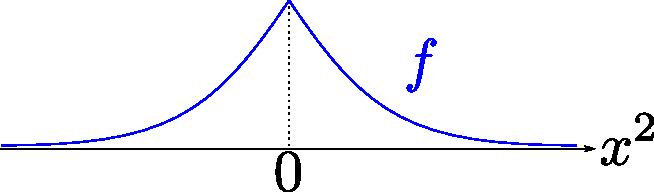
\includegraphics{localized.pdf}
  \caption{$Y$のところに局在した解の様子。$Y$から離れるにしたがって指数関数的に小さくなる。}
  \label{fig:localized}
\end{figure}



\subsection{domain-wallフェルミオンとAPS指数}
さて、domain-wallフェルミオンとAPS指数の関係について述べます。今、$X$を$Y$のところで2つに分け、$X_{+}$と、$X_{-}$で異なるSPT相にあるという状況を考えています。$X_{+}$の方をA相、$X_{-}$の方をB相と呼ぶことにしましょう。どちらが自明な相で、どちらが非自明な相かはスキームによります。今のようにPauli-Villarsで$\Lambda>0$の場合には、A相が非自明、B相が自明になります。ただし、スキームに依存しているというのは気持ち悪いので、$X$全体がB相になっているものとの比を考えることにします。\ref{subsec:massiveASindex}項の記号を使って
\begin{align}
  \frac{\ZDW}{Z(X,M)}=\frac{\det \HDW}{\det \Hp}\label{DWratio}
\end{align}
を考えます。

\ref{subsec:massiveASindex}項と同じ議論をすると\eqref{DWratio}の位相は
\begin{align}
  \frac{\ZDW}{Z(X,M)}=\qty|\frac{\ZDW}{Z(X,M)}|e^{\pi i \IDW},\qquad
  \IDW=\frac12 (\eta(\HDW)-\eta(\Hp))
\end{align}
となります。$\frac{\ZDW}{Z(X,M)}$は実数ですから$\IDW$は整数になります。これは、既に非自明な結果です。

今の系は\ref{subsec:anomalyinflow}項のシナリオを実現しているはずなので、$\Zt$と$\frac{\ZDW}{Z(X,M)}$は同じものだと期待できます。ただし、絶対値の部分はスキームによるので位相の部分だけを考えます。ここから
\begin{align}
  \IDW\equiv \Ind(\DAPS)\mod 2 \label{massiveAPSmod2}
\end{align}
となっていると予想します。ここで$\Ind(\DAPS)$は$X_{+}$において、その境界$Y$でAPS境界条件を考えた場合のAPS指数です。

\ref{subsec:massiveASindex}項での質量のあるフェルミオンとAS指数の場合のことを考えると、\eqref{massiveAPSmod2}よりも、さらに強い関係
\begin{important}
  \begin{align}
    \IDW=\Ind(\DAPS)\label{massiveAPSindex}
  \end{align}    
\end{important}
が成り立つことが予想できます。実際これが正しいことを\cite{Fukaya:2017tsq}で議論し、\cite{Fukaya:2019qlf}で証明を与えました。

証明の詳細はここでは述べませんが、証明は簡単ではないということを説明します。\eqref{massiveASindex}のときは$D$と$\Hm$が反交換することが効いていました。今の場合、質量項が定数でないために$D$と$\HDW$が反交換しません。なので、\eqref{massiveASindex}と同じ簡単な証明は今は出来ません。




\section{一般の次元}
これまで、1次元のアノマリーを2次元から見た描像について説明してきました。これは、任意の奇数次元のパリティアノマリーと呼ばれているアノマリーを1次元高い空間から見るという描像に一般化できます。

$n$を偶数とし、$X$を$n$次元多様体で\ref{subsec:spinorsetup}項で考えたような構造付きの多様体とします。また\ref{subsec:spinorsetup}項で考えたフェルミオン$\psi,\psib$とDirac演算子$D$と考えます。

まず、$X$を閉じた多様体として、質量のないフェルミオンの理論を考えます。作用は
\begin{align}
  S=\int_{X}d^n x \sqrt{g}\psib iD \psi
\end{align}
とします。この作用は軸性$\U(1)$変換
\begin{align}
  \psi\to \psi'=e^{i\gammab \alpha}\psi, \psib\to \psib'e^{i\gammab \alpha}
\end{align}
で不変です。しかし軸性$\U(1)$アノマリーがあり、積分測度は不変ではなく
\begin{align}
  D\psib' D\psi'=D\psib D\psi J,\quad J=e^{-2i\alpha \Ind(D)}
\end{align}
となります。ここで$\Ind(D)$は$D$のAS指数で$D\phi=0$のカイラリティ が$+$の解の個数を$n_{+}$、カイラリティ が$-$の解の個数を$n_{-}$として
\begin{align}
  \Ind(D):=n_{+}-n_{-}
\end{align}
と定義されます。AS指数定理は
\begin{align}
  \Ind(D)=\int_{X}\Tr(e^{\frac{F}{2\pi}})\Aroof(R)
\end{align}
と書けます。ここで$\Aroof(R)$は、Aルーフ種数と呼ばれ、次のように定義されています。$\omega^{a}{}_{b}=\omega_{\mu}{}^{a}{}_{b}dx^{\mu}$から作られる曲率$R$を
\begin{align}
  R^{a}{}_{b}=d\omega^{a}{}_{b}+(\omega\wedge \omega)^{a}{}_{b}
\end{align}
とします。$\omega\wedge \omega$は行列としての積で、かつ1形式同士の外積とします。$R$を局所的に2形式を値に持つ行列とします。Aルーフ種数は形式的に
\begin{align}
  \Aroof(A)=\sqrt{\det\frac{iR/(4\pi)}{\sinh iR/(4\pi)}}
\end{align}
と書けます。

$X$が境界がある場合のAPS指数定理も同様にあります。$X$の境界を$Y$として、$Y$の付近では$Y\times \Rb$になっているとします。ここで、$x^1,\dots,x^{n-1}$を$Y$の座標、$x^n$を$Y$に垂直な座標とします。うまく座標、ゲージをとることで$D\psi=0$という方程式は、
\begin{align}
  \del_{n}\psi=B\psi,\qquad B=-\gamma^{n}\gamma^{i}D_{i}
\end{align}
と書けます。APS境界条件は$Y$上で
\begin{align}
  \frac{B}{|B|}\psi=+\psi
\end{align}
を課します。これは、軸性$\U(1)$対称性を保ちます。APS指数定理は
\begin{align}
  \Ind(\DAPS)=\frac12 \eta(iD_{n-1})+\int_{X}\Tr(e^{\frac{F}{2\pi}})\Aroof(R)
\end{align}
となります。$D_{n-1}$は$Y$でのDirac演算子です。

質量のあるフェルミオンとAS指数の関係も同じです。$M>0$として
\begin{align}
  \Hm:=\gammab(D+M),\quad \Hp:=\gammab(D-M)
\end{align}
とします。このとき
\begin{align}
  \Ind(D)=\frac12\eta(\Hm)-\frac12 \eta(\Hp)
\end{align}
が成り立ちます。

質量のある場合のAPS指数の関係も同様にあります。$X$を$Y$のところで$X_{+}$と$X_{-}$の2つに分けます。$\kappa$を$X$上の関数で$X_{+}$で$+1$、$X_{-}$で$-1$、$Y$で$0$の値をとるとします。$\HDW$を
\begin{align}
  \HDW:=\gammab(D+M\kappa)
\end{align}
と定義します。$Y$を境界とする$X_{+}$で定義されたAPS境界条件のDirac演算子を$\DAPS$として、$M$が十分に大きいとき
\begin{align}
  \Ind(\DAPS)=\frac12 \eta(\HDW)-\frac12 \eta(\Hp)\label{massiveAPSgeneraldim}
\end{align}
が成り立ちます。


\section{展望}

今回は、奇数次元のパリティアノマリーと呼ばれているものに限って、それを1次元高い空間でのAPS指数からアノマリー流入で理解するという描像に限って説明しました。しかし、\cite{Witten:2015aba}では、フェルミオンに関するすべてのアノマリーは1次元高い空間からのアノマリー流入で理解できるということが述べられました。つまり、アノマリー流入がアノマリーの理解に関して、かなり本質的な役割を果たすということです。アノマリー流入はもともと\cite{Callan:1984sa}で発見され、様々な場面で重要な役割を果たしてきました。\cite{Callan:1984sa}ではdomain-wallだけでなく、4次元の中では弦、一般には渦糸と呼ばれるcodim 2のdefectについてもアノマリー流入があることを示しています。この渦糸や、他の様々なcodimensionのdefectとアノマリー流入について、現代的な観点からあらためて考察してみるというのは面白い課題だと思います。特に物性で研究されている高次トポロジカル物質との関係も気になるところです。

また、この講義では、Dirac演算子に限って説明しましたが、\cite{Fukaya:2019qlf}では、もう少し広いクラスの演算子を取り扱っています。偶数次元で1階の反エルミート楕円形微分演算子$D$と、それと反交換する$\gammab$がある場合に同様の定理が成り立つことが証明できています。もっと広いクラス、特に奇数次元の場合に拡張するのは1つの今後の課題です。

奇数次元の指数定理の1つの例として、$n=4k+1$次元でゲージ群が$\mathrm{SU}(2)$、あるいは$\mathrm{USp}(2r)$の場合のmod 2 指数と呼ばれているものがあります。これは、$4k$次元のWittenの大域的アノマリーと呼ばれているものと関係があり、物理でも興味ある対象です。これに関しては、やはりdomain-wallフェルミオンの見方ができることが分かって、論文を準備中です\cite{Fukaya:2020abc}。

今回は、物理のパリティアノマリーのアノマリー流入を考えたいという動機でAPS指数を考えたのですが、この動機からするとAPS指数そのものは必要なくて、その偶奇だけが必要でした。しかし、いろいろやってみると整数のAPS指数がdomain-wallフェルミオンの言葉で書けることが分かりました。このことの物理的意味をもう少し考えてみたいです。特に数学者の方々と共同研究をするようになって思うようになったことは、指数というのは既にかなり情報を捨て去っているということです。もちろん本当に物理的な情報、例えばDirac演算子のスペクトルそのものは、この方向では難しく、もっと定量的な解析が必要です。しかし、例えばK理論の元としての区別のような、もっときれいな部分に限っても指数以上のものがあるはずです。これらについて物理的観点から考えてみることは興味深い課題だと思います。

\appendix
\section{$\eta(iD_1)$の計算}\label{app:calceta}
この計算に必要なHurwitzゼータ関数についてまとめておきます。$\Re b>0$, $\Re s >1$のとき
\begin{align}
  \zeta(s,b):=\sum_{n=0}^{\infty}\frac{1}{(n+b)^s}
\end{align}
と定義します。また、それ以外の$s$にも解析接続で定義します。特に後に用いるのは$s=0$での値
\begin{align}
  \zeta(0,b)=\frac12-b\label{zeta0}
\end{align}
です。

$\eta(iD_1)$を定義にしたがって計算します。$\Re s$を十分大きいとして
\begin{align}
  \eta(iD_1,s):=\sum_{r\in \halfint}\frac{\lambda_{r}}{|\lambda_r|^{1+s}},\qquad \lambda_{r}=r+a
\end{align}
を計算していきます。これはゲージ変換$a\to a+1$で不変ですから
\begin{align}
  -\frac12 <a <\frac12
\end{align}
のときに計算すれば十分です。$b:=a+\frac12$とすると$0<b<1$です。この$b$を用いると
\begin{align}
  \eta(iD_1,s)=\sum_{n\in\Zb} \frac{n+b}{|n+b|^{1+s}}
  =\sum_{n=0}^{\infty}\frac{1}{(n+b)^s}+\sum_{n=1}^{\infty}\frac{-n+b}{|-n+b|^{1+s}}
\end{align}
となります。前の和は$\zeta(s,b)$そのものです。後ろの和は
\begin{align}
  &\sum_{n=1}^{\infty}\frac{-n+b}{|-n+b|^{1+s}}
  =-\sum_{n=1}^{\infty}\frac{n-b}{|n-b|^{1+s}}\nonumber\\
  &=-\sum_{n=0}^{\infty}\frac{n+1-b}{|n+1-b|^{1+s}}
  =-\sum_{n=0}^{\infty}\frac{1}{(n+1-b)^{s}}
  =-\zeta(s,1-b)
\end{align}
となります。
ですから
\begin{align}
  \eta(iD_1,s)=\zeta(s,b)-\zeta(s,1-b)
\end{align}
を得ます。

$\eta(iD_1)=\eta(iD_1,s=0)$を\eqref{zeta0}を用いて
\begin{align}
  \eta(iD_1)=\frac12-b-\qty(\frac12 -(1-b))
  =1-2b=-2a,\qquad (-\frac12 < a <\frac12)
\end{align}
となります。

一般の$1/2$の奇数倍でない$a$の場合、四捨五入したもの$[a+1/2]$を引くことにより
\begin{align}
  -\frac12 <a-[a+1/2]<\frac12
\end{align}
を満たすので、
\begin{align}
  \eta(iD_1)=-2(a-[a+1/2])=2[a+1/2]-2a
\end{align}
を得ます。

\bibliographystyle{utphys}
\bibliography{ref}
\end{document}